%%%%%%%%%%%%%%%%%%%%%%%%%%%%%%%%%%%%%%%%%%
%%%%%%%%%%%%%                 %%%%%%%%%%%%
%%%%%%%%%%%%%    EXERCISE 1   %%%%%%%%%%%%
%%%%%%%%%%%%%                 %%%%%%%%%%%%
%%%%%%%%%%%%%%%%%%%%%%%%%%%%%%%%%%%%%%%%%%
\begin{exercise}[]{
    Consider the following snapshot of a system:
    
    \begin{figure}[h]
        \begin{center}
            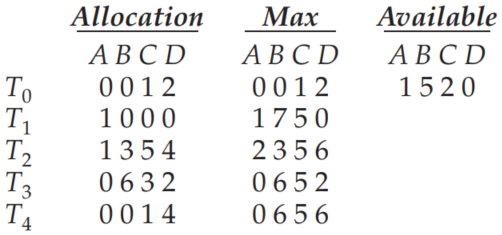
\includegraphics[scale=1]{fig8.3.png}
        \end{center}
    \end{figure}

    Answer the following questions using the banker algorithm:
    
    
    \begin{enumerate}
        \item [a)]
    What is the content of the matrix Need?
    
    \item [b)]
    Is the system in a safe state?
    
    \item [c)]
    If a request from thread $T_1$ arrives for (0,4,2,0), can the request be
    granted immediately?
    \end{enumerate}
    }
  \begin{solution}
  \par{~}
  \begin{enumerate}
      \item The need matrix is shown in Figure \ref{1-1}
       \begin{table}[h]
         \centering
        \begin{tabular}{lllll}
        \hline
           & A & B & C & D \\ \hline
        T0 & 0 & 0 & 0 & 0 \\
        T1 & 0 & 7 & 5 & 0 \\
        T2 & 1 & 0 & 0 & 2 \\
        T3 & 0 & 0 & 2 & 0 \\
        T4 & 0 & 6 & 4 & 2 \\ \hline
        \end{tabular}
        \caption{Need matrix \label{1-1}}
        \end{table}
      \item Yes. The sequence can be $\langle T_0 (1,5,3,2), T_3 (1,11,6,4),T_4 (1,11,7,8),T_2(2,14,12,12),T_1(3,14,12,12)\rangle$, where the numbers in the parenthesis are the available resources after the thread is terminated.
      \item Check that $(0,4,2,0)\le(1,7,5,0)$ and $(0,4,2,0)\le(1,5,2,0)$. We can make a virtual allocation to $T_1$, at this moment, the available vector will be $(1,1,0,0)$ and the need matrix will be Figure \ref{1-2}
      \begin{table}[htbp]
        \centering
        \begin{tabular}{lllll}
        \hline
           & A & B & C & D \\ \hline
        T0 & 0 & 0 & 0 & 0 \\
        T1 & 0 & 3 & 3 & 0 \\
        T2 & 1 & 0 & 0 & 2 \\
        T3 & 0 & 0 & 2 & 0 \\
        T4 & 0 & 6 & 4 & 2 \\ \hline
        \end{tabular}
        \caption{Need matrix \label{1-2}}
        \end{table}
        We can find a sequence $\langle T_0 (1,1,1,2), T_2 (2,4,6,6),T_1 (3,8,8,6),T_3(3,14,11,8),T_4(3,14,12,12)\rangle$ to ensure the safety condition. The request will be immediately granted.
    
  \end{enumerate}
  \end{solution}
  \label{ex1}
\end{exercise}

\newpage

%%%%%%%%%%%%%%%%%%%%%%%%%%%%%%%%%%%%%%%%%%
%%%%%%%%%%%%%                 %%%%%%%%%%%%
%%%%%%%%%%%%%    EXERCISE 2   %%%%%%%%%%%%
%%%%%%%%%%%%%                 %%%%%%%%%%%%
%%%%%%%%%%%%%%%%%%%%%%%%%%%%%%%%%%%%%%%%%%
\begin{exercise}[]{Consider the following snapshot of a system:
    \begin{figure}[h]
        \begin{center}
            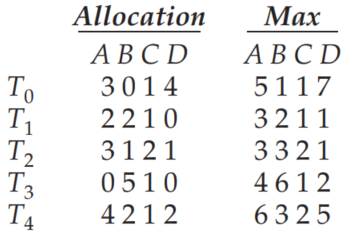
\includegraphics[scale=1]{fig8.9.png}
        \end{center}
    \end{figure}
    
    Using the banker algorithm, determine whether or not each of the following states is unsafe. If the state is safe, illustrate the order in which the threads may complete. Otherwise, illustrate why the state is unsafe.
    \begin{enumerate}
        \item [a)]
    Available = (0, 3, 0, 1)
    \item [b)]
    Available = (1, 0, 0, 2)
    \end{enumerate}
    
    }
  \begin{solution}
  \par{~}
  The need matrix is shown in Table \ref{2-1}

  \begin{table}[ht]
    \centering
    \begin{tabular}{lllll}
    \hline
       & A & B & C & D \\ \hline
    T0 & 2 & 1 & 0 & 3 \\
    T1 & 1 & 0 & 0 & 1 \\
    T2 & 0 & 2 & 0 & 0 \\
    T3 & 4 & 1 & 0 & 2 \\
    T4 & 2 & 1 & 1 & 3 \\ \hline
    \end{tabular}
    \caption{Need Matrix \label{2-1}}
    \end{table}
    \begin{enumerate}
        \item First, only $T_2$ can be selected as the first thread in the safety sequence. The available resources for later threads are $(3,4,2,2)$. Then only $T_1$ can be selected. After $T_1$ release its resources, the available vector will be $(5,6,3,2)$. Now $T_3$ can be added to the sequence, making the available vector become $(5,11,4,2)$. However, neither $T_0$ nor $T_4$ can be added to the sequence for lack of $D$ resource. The state is unsafe.
        \item The state is safe. We can find a sequence $\langle T_1 (3,2,1,2), T_2 (6,3,3,3),T_3 (6,8,4,3),T_4(10,10,5,5),T_0(12,11,5,8)\rangle$ to ensure the safety condition.
    \end{enumerate}
  \end{solution}
  \label{ex2}
\end{exercise}

\newpage

%%%%%%%%%%%%%%%%%%%%%%%%%%%%%%%%%%%%%%%%%%
%%%%%%%%%%%%%                 %%%%%%%%%%%%
%%%%%%%%%%%%%    EXERCISE 3   %%%%%%%%%%%%
%%%%%%%%%%%%%                 %%%%%%%%%%%%
%%%%%%%%%%%%%%%%%%%%%%%%%%%%%%%%%%%%%%%%%%
\begin{exercise}[]{Which of the six resource-allocation graphs shown in below illustrate deadlock? For those situations that are deadlocked, provide the cycle of threads and resources. Where there is not a deadlock situation, illustrate the order in which the threads may complete execution.   
    \begin{figure}[h]
        \begin{center}
            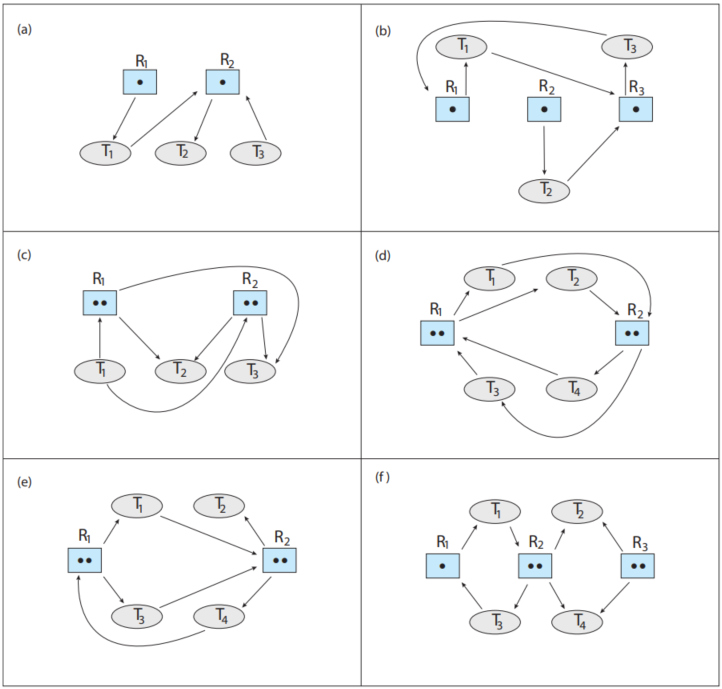
\includegraphics[scale=1]{fig8.18.png}
        \end{center}
    \end{figure}
    }
  \begin{solution}
  \par{~}
  \begin{enumerate}
      \item[a)] Not a deadlock. After $T_2$ terminates, either $T_1$ or $T_3$ can access $R_2$ and terminates. Then the remained threads can also terminate.
      \item[b)] Is a deadlock, formed by $R_1$, $T_1$, $R_3$, $T_3$.
      \item[c)] Not a deadlock.  $T_3$ and $T_2$ have gained their resources and can terminate. After that, $T_1$ can access the resource and terminate.
      \item[d)] Is a deadlock, formed by $T_1,R_2,T_3,R_1$ and $R_1,T_2,R_2,T_4$
      \item[e)] Not a deadlock. $T_2$ terminates first. Then $T_1$ can get the resource released by $T_2$ and terminate. Finally, $T_3$ and $T_4$ can both access the resources and terminate.
      \item[f)] The graph is invalid, since there are only two instances for $R_2$ but three instances are assigned to different threads. 
  \end{enumerate}
  \end{solution}
  \label{ex3}
\end{exercise}